\documentclass[12pt,a4paper, twocolumn]{article}
\usepackage[utf8]{inputenc}
\usepackage[english]{babel}
\usepackage{amsmath}
\usepackage{amsfonts}
\usepackage{amssymb}
\usepackage{graphicx}
%\usepackage[left=2cm,right=2cm,top=2cm,bottom=2cm]{geometry}
\usepackage{lipsum}
\usepackage{multicol}
\usepackage{float}

\floatstyle{boxed}
\restylefloat{figure}
\setlength\columnsep{20pt}

\author{Baptiste \textsc{Rouger} \and Fanny \textsc{Roussel}}
\title{Report :\\Experimental Methods}
\date{February 20$^{\text{th}}$, 2017}

\begin{document}
\maketitle

\begin{abstract}
Cryptobiosis is the phenomenon that consists in slowing down the metabolism of an organism in order to extend its life. This phenomenon can be studied in small multicellular organisms that are able to do it : tardigrads. We studied the time required to set up this state in \textit{Hypsibius dujardini}. We have been able to show that, with an increasing concentration of NaCl, the average time required to observe half of the tardigrads in cryptobiosis state was decreasing accordingly. Furthermore, we show that the higher the stress, the harder it is to implement cryptobiosis. Study this mecanism could help to improve cryogenesis, which is currently used to preserve model organisms like bacterias from aging.
\end{abstract}

%\begin{multicols}{2}



\section{Introduction}
Tardigrades (species : Hypsibius Dujardini) are small animals known in the literature as capable of resisting extreme conditions. They have the ability to enter into cryptobiosis in order to protect themselves from temperature variations (cryobiosis), dehydration (anhydrobiosis), lack of oxygen (anoxybiosis) or high salt concentrations (osmobiosis). Confronted to a stress, tardigrades are entering a reversible suspended  and contracted metabolic state, losing more than 95\% of their water and secreting trehalose, a sugar aimed at protecting their cells. Once back in a friendly environment, tardigrades can get out of the tun conformation, generally after a few hours, and behave normally again.
The aim of our project was to observe tardigrades confronted to different intensities of a specific stress, and their response over time in terms of tun formation or death. We decided to put our cultured tardigrades in different concentrations of NaCl – one of the stress they are known to be able to resist to – and observe the evolution of the population : we knew that if tardigrades are confronted to a stress, they need to protect themselves. If not, they die. Our protocol was thus to inject a certain quantity of NaCl solution in the tardigrades’ environment and track the population behaviour every two minutes until no tardigrade is moving in the observed sample anymore : they would either be in tuns or dead. Our result would show if there is a threshold at which tardigrades are exposed too violently to the stress and do not have enough time to transform into tun. In this situation, our population would die, instead of forming tuns. We also wanted to determine if there is a link between the concentration of NaCl in the environment and the time at which we can observe the first tuns : is the intensity of the stress influencing the tun formation speed itself? All these measurements would allow us to understand better how an organism can protect itself to the point that a pretty sensitive animal can become almost indestructible.

\section{Methods}
In order to test the effect of the concentration of salt on the time of conformation change (from active behaviour to tun conformation) of  the tardigrades, we needed to create our own multiwell plates. Indeed tardigrades are small and mobile animals, swimming in the solution that we bought. In order to be able to count them, we had to use wells with a really small depth- in which we could still observe tens of them. The multiwell plates we created (c.f. DIY \textsc{Section}) were composed of ten wells, that we filled each time with 5 $\mu$L of the solution of cultured tardigrades, and 5 $\mu$L of a solution of NaCl. As the solution in which we received the tardigrades was not salty, the 5$\mu$L of NaCl solution was concentrated twice the concentration we wanted to obtain. For instance, when we wanted to observe the behaviour of tardigrades put in 0.1M of NaCl, we were putting  5 $\mu$L of the tardigrade solution with 5 $\mu$L of NaCl solution at 0.2M in our wells.
Our protocol was as follow : we set one well only containing 5 $\mu$L of the solution of cultured tardigrades under the microscope and counted out loud the number of living, dead and tun tardigrades we could observe to make sure we had enough animals in the well to get significative results. A second person was always taking notes of the count. Once we were sure to have a sufficiently large population in the sample, we injected the 5$\mu$L of NaCl solution. This was time t=0. We then counted every two minutes the number of living, dead, and tun tardigrades (\textsc{Figure} 1), until no tardigrade was moving in the well. We observed our samples on a maximal length of 50 minutes, with a last measurement at 60 minutes. Though, when we observed no moving tardigrad during 6 consecutive minutes, we stopped the count, considering all the animals were in tun or dead, and that their state would not evolve anymore. We only stopped the count when we obtained similar numbers of inactive tardigrades (dead, tun) 3 times in a row, while no active one was remaining.
Moreover, in order to compensate the water lost by evaporation, we were refilling the well to 10 $\mu$L at 30 minutes, when the experiment was lasting that long : as tardigrades are also known to protect themselves from dehydration, we did not want them to face another kind of stress. Moreover, evaporation would have increased the solution salt concentration.\\
We experimented on the tardigrades with different concentrations of NaCl : $0.000$M, $0.050$M, $0.065$M, $0.080$M and $0.100$M. Everytime, we tried to observe at least a hundred of tardigrades, over 2 or 3 60 minutes of counting, for each observed concentration. \\

Once we had all our results, we developed several indexes to represent the number of living, tun, and dead tardigrades. The first one is the proportion of one category of tardigrad over the whole population $\frac{\text{Active, Tun or Dead}}{\text{Whole population}}$. The second index represents the proportion of tun tardigrades over the living population $\frac{\text{Tun}}{\text{Tun}+ \text{Active}}$. With these, we can represent the kinetics of the number of tardigrades that are active, in tun, or dead. In other words, active tardigrades, once confronted to NaCl, have two options : they can either transform in tuns or die. We should thus observe the number of active tardigrades progressively splitting in the two other categories, taking into account that there can already be some dead or tun tardigrades at t=0.\\

In order to represent the tun conformation speed better, we created a last index, which is the half-time to conformation change ($tcc_{1/2}$), which represents the time at which half of the living (active + tun) tardigrades are in the tun conformation. With this index, we can have a representation of how fast do the tardigrades change of conformation, from their active form to osmobiosis.


\setcounter{figure}{0}
\begin{figure}
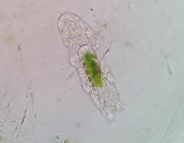
\includegraphics[width=\linewidth]{dead.png}
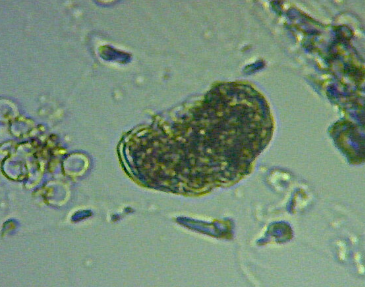
\includegraphics[width=\linewidth]{tun.png}
The tardigrade conformations showed by these pictures are our bases to determine in which states they are. On the left, the tardigrade is dead : we observe a relaxed conformation and no movement. After a few minutes, the dead tardigrade seems to begin dissolving in the environment. On the right, the tardigrade is in tun : we observe a dense ball shape, and no movement. Finally, when the tardigrades are still moving, swimming, or eating, we consider that they are active.
\label{dead-tun}
\caption{The different tardigrades' conformations}
\end{figure}


\section{Results}

Figure 2 shows the evolution of a tardigrade sample over time, when no NaCl has been put in their environment. This is our control experiment. We can observe on \textsc{Figure} 2 (top graph) that the proportion of dead tardigrades is constant, despite noisy errorbars. We can observe the same thing with the proportion of active tardigrades. The noise we observe on these curves will be discussed in the Discussion \textsc{Section}. Moreover, we observe no conformation change for any tardigrade, as the proportion of tun stays at 0 during the whole experiment.\\
This control experiment allows us to say that the fact that we place tardigrades in the wells and under the microscope does not disturb them as they do not die nor form tun. After having made sure that no tardigrade was dying or transforming in absence of stress, we could permorm our experiments with increasing concentrations of NaCl.\\



\begin{figure}
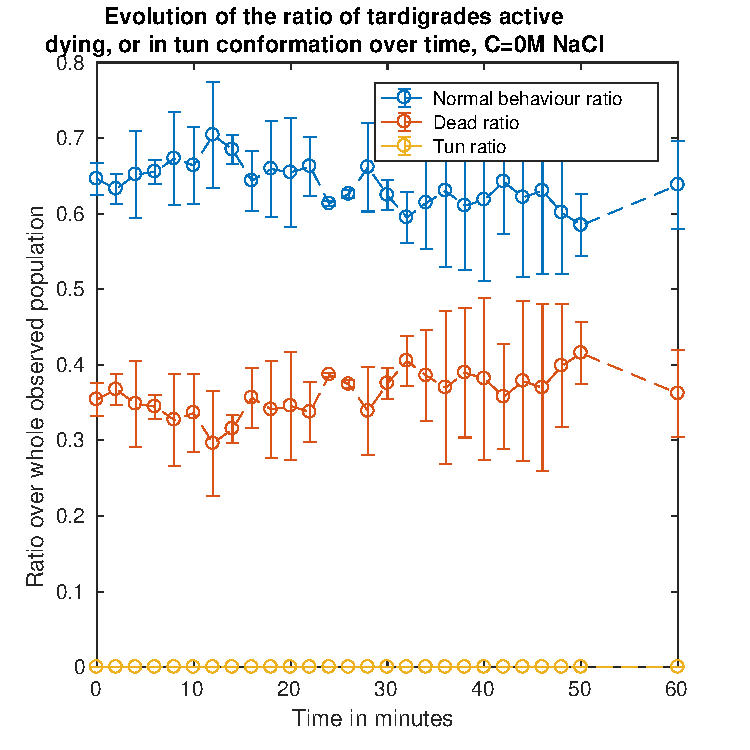
\includegraphics[width=\linewidth]{000.pdf}
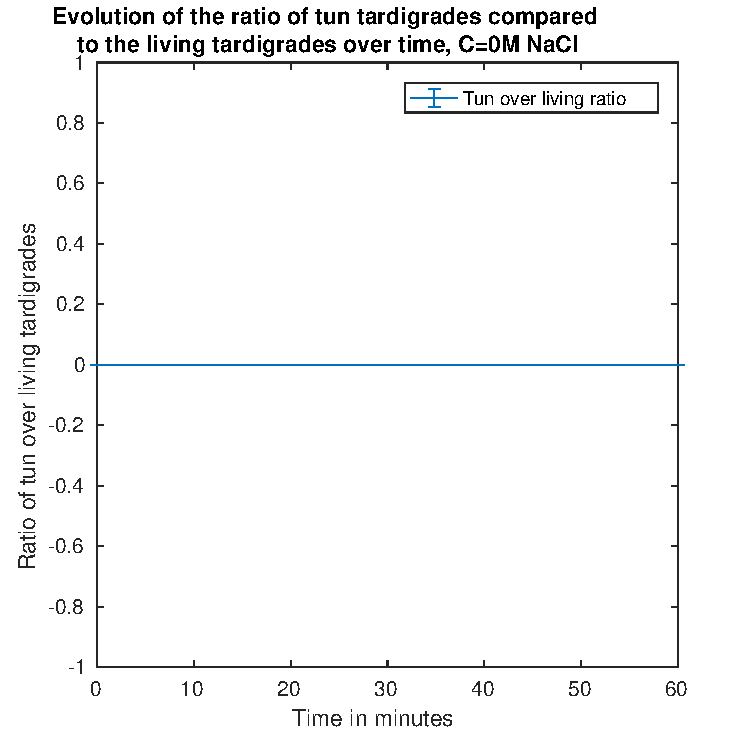
\includegraphics[width=\linewidth]{000t.pdf}
\label{fig000}
We can see in this figure that the proportion of each class (active, dead or tun) of tardigrade is not significantly changing with time. On the proportion of tun over living ($T/L$) graph, we can see that no tardigrade is going into osmobiosis at this concentration.
\caption{Kinetics of the number of active, tun and dead tardigrads at 0M of NaCl}
\end{figure}


The first concentration of NaCl we tested was $0.050$M. \textsc{Figure} 3 shows the kinetics of the conformation change for this concentration (top graph). On these graphs, we can first observe that the number of tardigrades that die during the experiment do not seem to change. However, we can observe an important change in the proportions of active and tun tardigrades : the number of active tardigrades is decreasing significantly, and the proportion of tun tardigrades is increasing accordingly.\\
Furthermore, we can oberserve on the graph of the evolution of the proportion of tun tardigrades over the living population (bottom graph) that this proportion is increasing significantly over time. Moreover, at $t=60$ minutes, we were still able to observe active tardigrades as the proportion of tun over living ($T/L$) is not $1$. This seems to show that we would need longer kinetics. This point will be discussed in the Discussion \textsc{Section}.\\
We can see that these graphs show much noise, with quite big error bars and a shaky curve. This might be the result of human error or due to the fact that we observe a wide variation of behaviour of the tardigrades at this concentration that is perhaps not so restrictive.

\begin{figure}
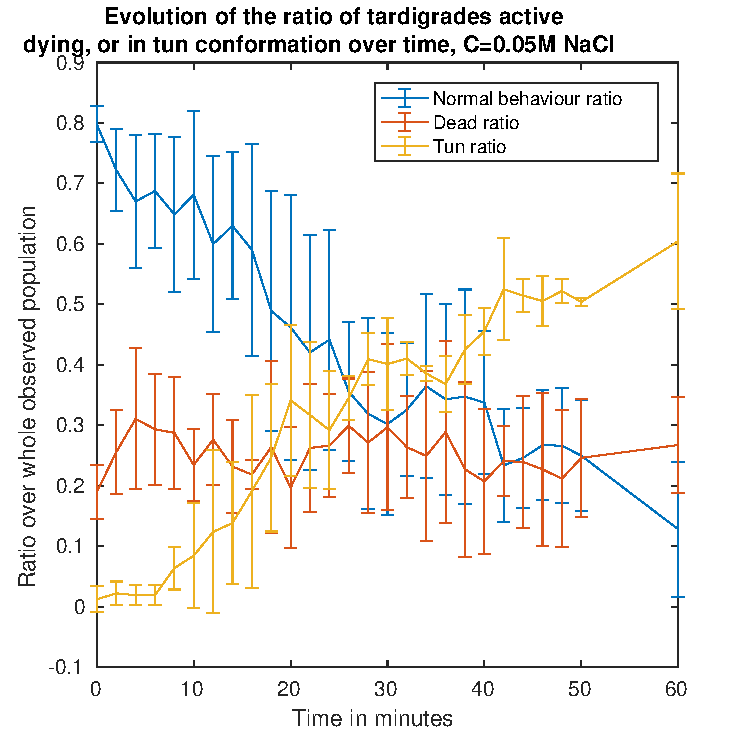
\includegraphics[width=\linewidth]{005.pdf}
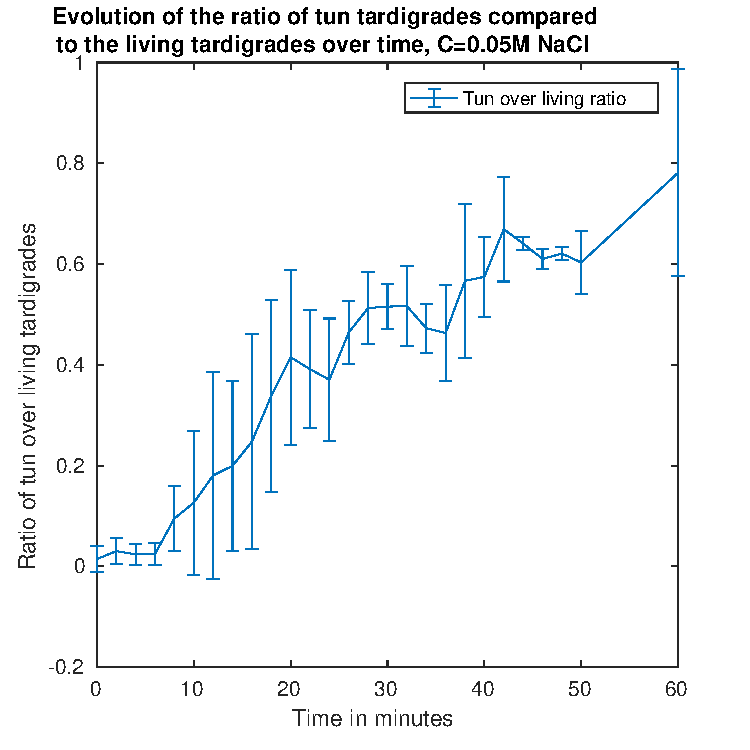
\includegraphics[width=\linewidth]{005t.pdf}
\label{fig005}
We can observe in this figure that the proportion of dead tardigrades is not increasing with time, whereas the proportion of active tardigrades is decreasing and the proportion of tun is increasing accordingly.\\ We also observe an increasing proportion of $T/L$ that seems to be still increasing at $t=60$ minutes around $0.8$.
\caption{Kinetics of the number of active, tun and dead tardigrads at 0.050M of NaCl}
\end{figure}


The second concentration that was tested is $0.065$M of NaCl. The kinetics of this concentration are presented in \textsc{Figure} 4. We can observe on the first graph that the proportion of dead tardigrades does not seem to increase . Though, we still observe that the proportion of active tardigrades is decreasing over time, falling to $0$ at around $t=26$ minutes. We observe a proportion of tun tardigrades increasing accordingly, with a plateau around $0.65\%$ at 20 minutes. We can also notice that the proportion of tardigrades in tun before 5 minutes is 0, which seems to indicate that the tardigrades need some time to detect the NaCl and change their conformation.\\
We also observe on the $T/L$ proportion graph (bottom part of the Figure) that the tardigrades seem to change their conformation faster or sooner than at $C=0.05$M, as the slope of the curve is steeper.\\
At this concentration, we observe that the proportion of $T/L$ is $1$ at $t=25$ minutes.

\begin{figure}
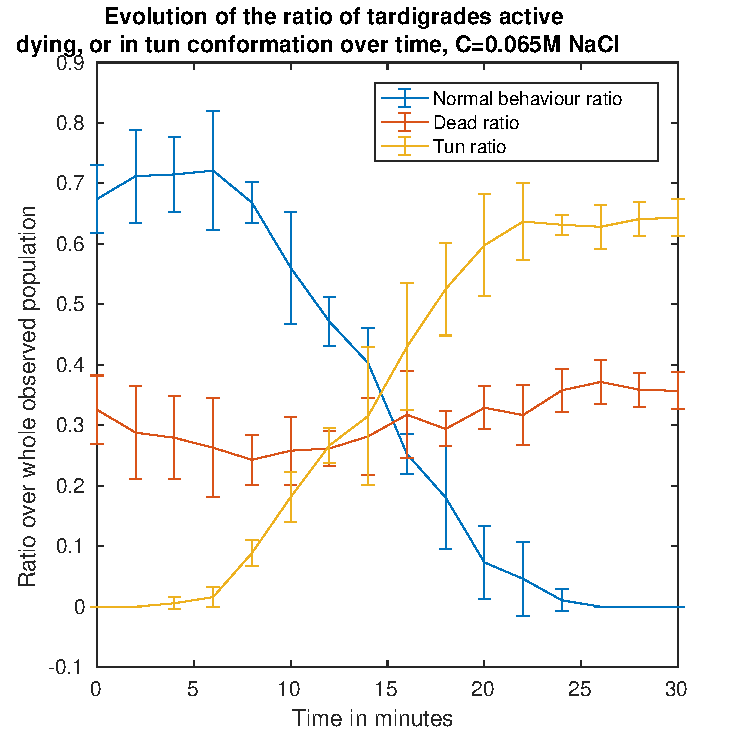
\includegraphics[width=\linewidth]{065.pdf}
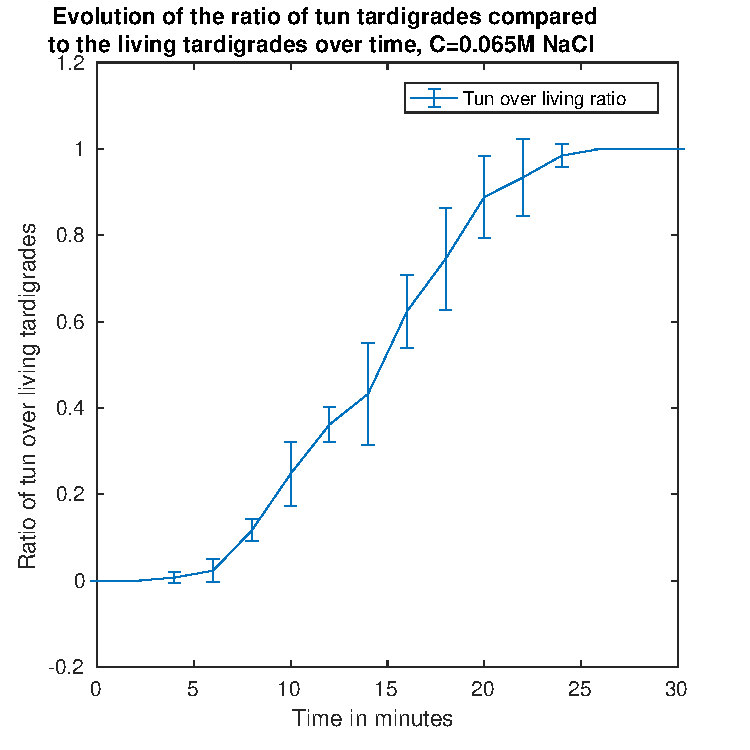
\includegraphics[width=\linewidth]{065t.pdf}
\label{fig065}
At this concentration, we do not observe an increasing proportion of dead tardigrades. Though, we observe an increasing proportion of tun tardigrades as the active one is decreasing.\\
We also observe that the $T/L$ proportion curve is steeper than for $C=0.05$M, and that we reach a proportion of $1$ at $t=25$ minutes.
\caption{Kinetics of the number of active, tun and dead tardigrads at 0.065M of NaCl}
\end{figure}


At a concentration of NaCl of $0.08$M (\textsc{Figure} 5), we see a behaviour similar to the one we get at 0.065M of NaCl, as the shapes of the curves look the same. The major difference that must be pointed out is that we show an increasing proportion of dead tardigrades ($+0.1$). This indicates that at this concentration, the tardigrades begin to die rather than go in tun as they die during the experiment. It might be due to the fact that they do not have time to adapt their metabolism and protect themselves against a too violent stress. \\
Although, we can still observe that the proportion of tardigrades in tun conformation is higher than the proportion of dead ones, so most of the tardigrades survive at this concentration.\\
Moreover, if we look at the $T/L$ proportion graph (bottom of the figure), we can observe that the conformation change starts sooner than at $0.065$M NaCl, as we observe the first tuns at around $t=4$ minutes. The plateau is reached at around $t=18$ minutes, which shows an even steeper slope than at $0.065$M NaCl. Thus, the tardigrades are going in tun conformation faster (or sooner) at this concentration.
\begin{figure}
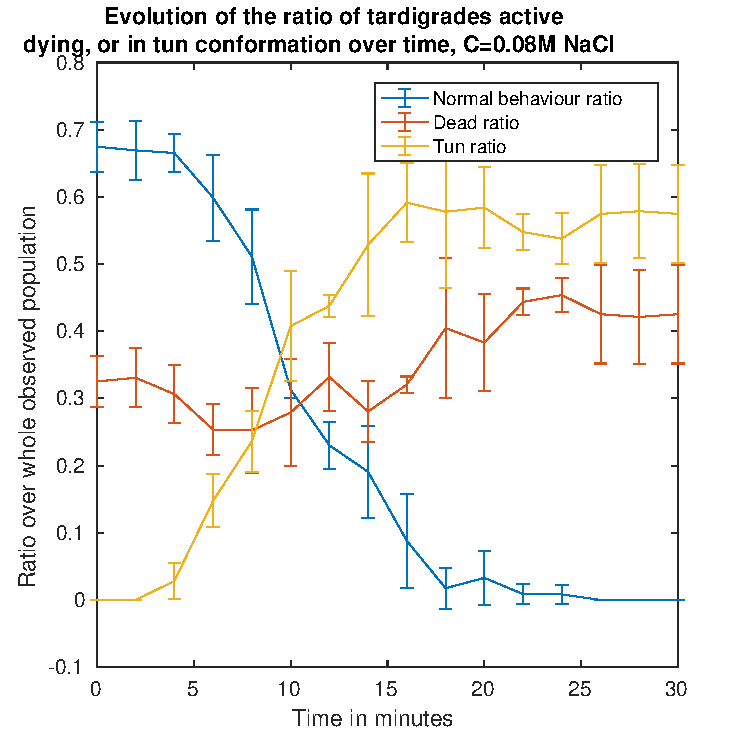
\includegraphics[width=\linewidth]{008.pdf}
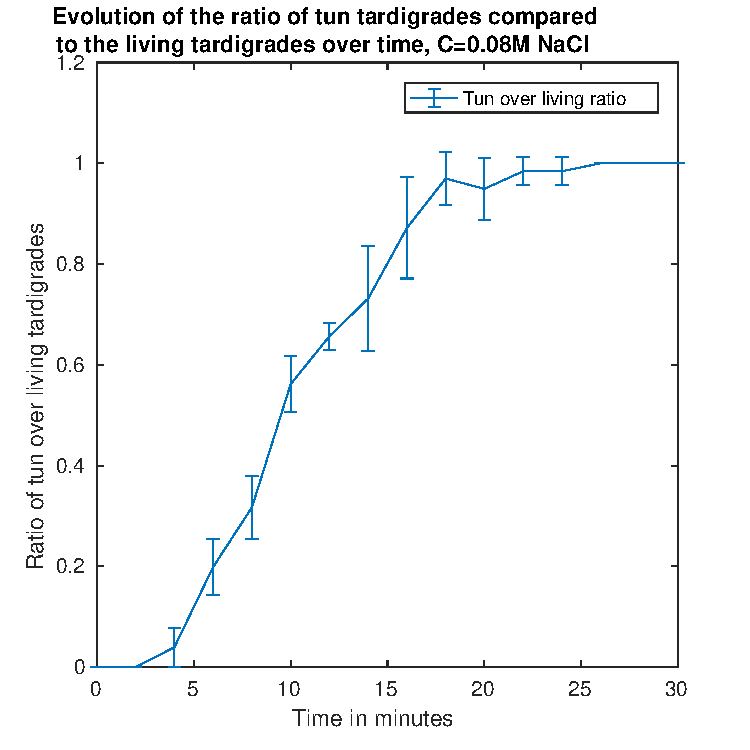
\includegraphics[width=\linewidth]{008t.pdf}
\label{fig008}
We observe at this concentration an increasing proportion of dead tardigrades, so some of them are diying during the experiment. We also observe a quickly increasing proportion of tun tardigrads and a decreasing proportion of active tardigrads. The $T/L$ proportion graph shows that the conformation change is happening sooner and/or faster, at it starts at $t=4$ minutes and reaches a plateau at $t=18$ minutes.
\caption{Kinetics of the number of active, tun and dead tardigrads at 0.080M of NaCl}
\end{figure}


The last concentration we experimented is $0.1$M NaCl.  The kinetics of this concentration are presented in \textsc{Figure} 6. We can observe that the porportion of dead tardigrades is strongly increasing at this concentration ($+0.25$). This shows that this concentration kills the tardigrades. Though, we can still observe that the proportion of tun tardigrades is also increasing, as it reaches a plateau at  around $0.5$ at $t=26$ minutes.\\
On the $T/L$ proportion graph, we show that the proportion of $T/L$ tardigrades is still increasing. It starts sooner than at $0.08$M NaCl (at $t=2$ minutes), but the slope is less steep, as the plateau is reached later (at $t=24$ minutes). We could therefore think that if the concentration is too high, it is less easy to the tardigrades to go in tun conformation, or that some of them are somehow less sensitive to this concentration. This phenomenon should be investigated further.

\begin{figure}
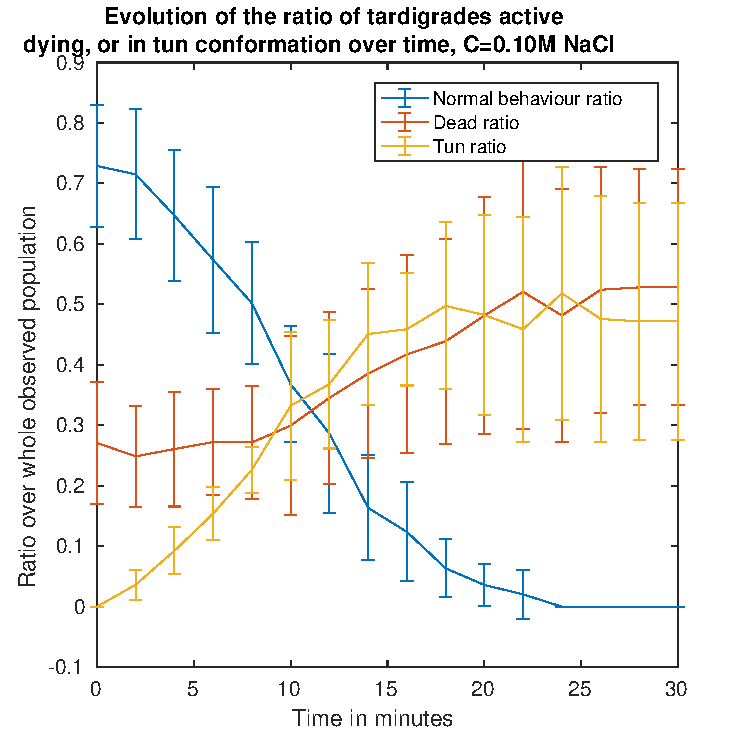
\includegraphics[width=\linewidth]{010.pdf}
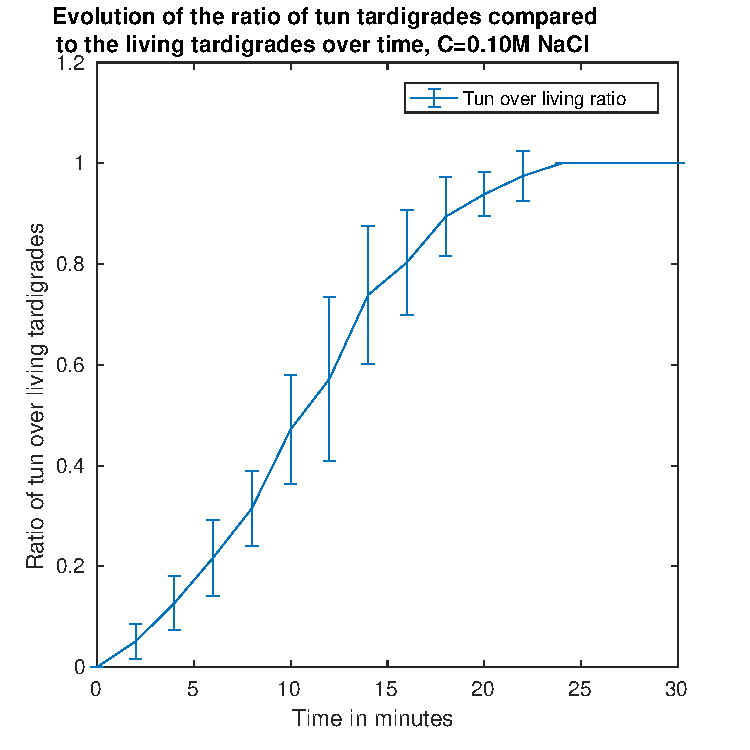
\includegraphics[width=\linewidth]{010t.pdf}
\label{fig010}
At $0.10$M NaCl, we show a strongly increasing proportion of dead tardigrades. We also show an increasing proportion of tun tardigrades, reaching a plateau around $0.5$, at $t=24$. We show that, even if the conformation change starts sooner for some of the tardigrades, it is happening later and or slower for some other tardigrades.
\caption{Kinetics of the number of active, tun and dead tardigrads at 0.100M of NaCl}
\end{figure}


To study the kinetics of the conformation change, we used a tool inspired from Chemistry : the half time ($t_{1/2}$), which is the time at which half of the quantity of the final species is obtained. Here, we get the half-time of conformation change ($tcc_{1/2}$) when half of the living tardigrades (active + tun) are in the tun conformation. We present the results in the \textsc{Figure} 7.\\
We can see that, with increasing concentration, the $tcc_{1/2}$ is decreasing. We can point out that we removed the point at $C=0.000$M NaCl on the graph as we had no tun tardigrades. We can observe that at $C=0.100$M NaCl, the $tcc_{1/2}$ is higher that at $C=0.08$M NaCl. This might be only due to noise, as we count the tardigrads every 2 minutes.\\
We can say from this figure that we have a relation between the concentration of NaCl of the environment and the $tcc_{1/2}$, which is linked to the speed of conformation change. However, we cannot conclude on the nature of the link between concentration and $tcc_{1/2}$.\\

\begin{figure}
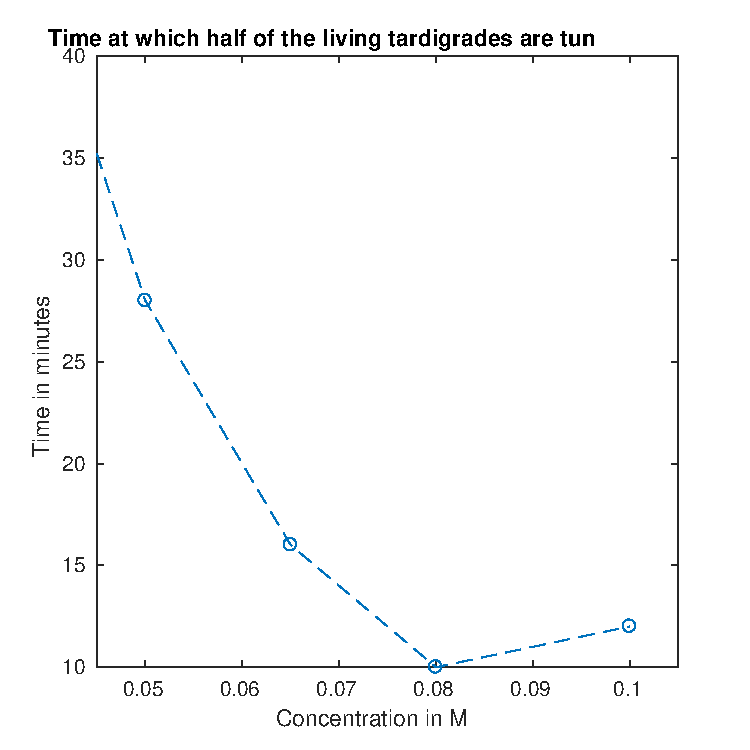
\includegraphics[width=\linewidth]{tcc.pdf}
\label{tcc}
We show on this figure the time at which half of the living tardigrades are in the tun conformation. We can observe that the higher the concentration, the faster the tardigrades are going in tun.
\caption{Half time of conformation change}
\end{figure}


\section{Discussion}
We learn from these results that there seem to be a correlation between the intensity of stress and the time at which tardigrades transform into tuns, but also that the higher the concentration of NaCl, the more dead tardigrades there are, in proportion. We wanted to make our results more reliable by swapping, for each counting session, between the role of counter and the role of note taker. For instance, if we had to count 3 times 40 minutes for a certain concentration, one person was counting twice, and the other was counting the third time. For the next session, the one who had only counted once would count more than the other. Our goal doing so was to give an accurate overview of the population behaviour, but it also created some noise, as two people are not observing the same way. The hardest part was to determine the threshold between active and tun states: at some point, tardigrades were stopping swimming, and beginning forming a ball, but keeping moving their legs and contort themselves. It is probable that both counters were not considering these intermediary states the same way and all the time, even more because we had to count very fast (around 40 tardigrades in 2 minutes). As we did not have much time to determine if one tardigrade was actually moving a bit, there could have been some leaps. Moreover, tardigrades are swimming in the well, from one depth to another, in 3 dimensions, which is difficult to track with the microscope.\\

For all these reasons, we decided to represent our results as ratios : the proportion of observed active tardigrades over the observed population at each timepoint. For instance, if at t=8 min, the counter has counted 43 tardigrades, with 24 active ones, 12 dead ones and 7 tuns, and at t=12, we have only seen 35 tardigrades, we can still compare the obtained values by taking into account the proportion of each state (active, dead, tun) over the observed population at a certain time, supposing that in average, we can observe the same proportion of tardigrades in each state (c.f. \textsc{Section} Methods). This is an important commitment, that needs to be taken into account when reading our results.\\

We also noticed that the size of the tardigrades was playing a role. Indeed we have been thinking that smaller animals were transforming faster and resisting better to the stress, while bigger ones were contorting themselves and often dying before being able to transform. Keeping that in mind, we have sampled 199 tardigrades and measured them using the ImageJ software to get precise measures, in order to have an idea of the size distribution of the population (see \textsc{Figure} 8). It would be interesting to work further on the impact of the size of the tardigrades on their reaction to a stress.\\

\begin{figure}
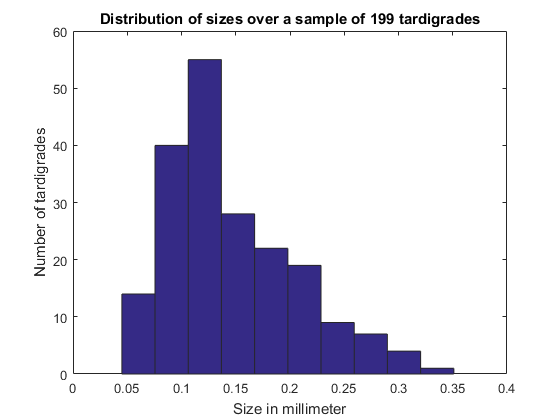
\includegraphics[width=\linewidth]{pop.png}
\label{pop}
We present here the size distribution of the population of tardigrades we experimented on. We can see that most of them measure around $0.1$mm.
\caption{Half time of conformation change}
\end{figure}


It is also important to take into account the fact that we only had two weeks time to run our experiments. If we had had more time, we would have wished to run these experiments for more concentrations. Indeed, we do not have any data between 0.0M and 0.05M. The concentrations in between are the one requiring the more time, as we do not know how long it can take for the sample to transform into tuns when confronted to a really small concentration of NaCl : it could take hours. This is what we would have wished to check, if we had had more time.\\

Automatizing the whole counting process would also have been a way to improve our results. However, as tardigrades are crushed by coverslips and moving to different depths when put into wells, it seems difficult to implement. With the material we had, it was impossible to catch them one by one with a micropipette in order to align them on a slide, as we planned to do at first. \\

We also wanted to work with a different type of stress, like cold, in order to wider our conclusions. Maybe the nature of the stress also makes the difference, in terms of tun conformations and tardigrade survival.\\

\section*{Conclusion}
Our work shows that the intensity of the stress tardigrades are confronted to has an impact on the future of these small animals. Indeed, if the stress -here, the concentration of salt- is too brutal, most of the tardigrades will die before being able to protect themselves with the tun conformation. When the concentration is not that high, it still determines the speed at which the tardigrades transform into tuns. For concentrations varying from 0.05 M to  0.1 M, we observed the first waves of tun formations from around 8 minutes to around 20 minutes. One explanation that can be given to the observed phenomenon is that, as tardigrades need to remove water from their organism in order to perform the tun transformation (c.f. Introduction \textsc{Section}), this process is accelerated by a high - but not too high - concentration of salt that increases osmotic pressure. This is, among others, another food for thought.


\newpage


\section*{DIY}
We could not efficiently count the tardigrades on normal slides : these animals are often swimming and known as not liking being observed under a coverslip. We did not want to influence too much the way they behave, and decided to create our own well plates. Our objective was to fix pipette tip frames on microscope slides. At the origin, we thought that tardigrades were very resistant animals, even in their active conformation. We have discovered that if these animals are known to survive almost any stress as tuns, they are indeed quite sensitive while out of this conformation : we first fixed our frame using nail polisher, directly available in the laboratory. We obtained watertight wells, able to contain the desired volume of solution. However, running our first experiments, we observed that an important proportion of tardigrades was dead or dying in a few minutes. He thus think that tardigrades do not resist acetone, even in such small concentrations. Our final multiwell plates were sticked to the slide with candle wax (see \textsc{Figure} 9).\\

It is also important to notice that we tried to concentrate the solution in which tardigrades were living, by centrifuging it. We tried several lengths (1 to 6 minutes) and speed (3k, 4k, 4.5k, 6k tour/minute), and always observed a high rate of dead tardigrades - sometimes, no living ones at all in the sample. We thus think that active tardigrades do not resist centrifugation.

\begin{figure}
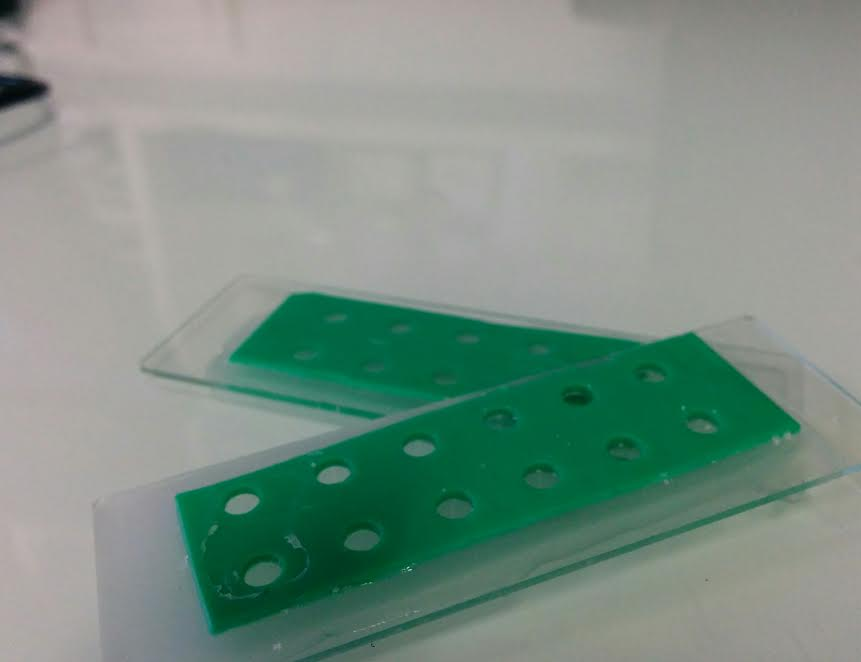
\includegraphics[width=\linewidth]{plates.png}

\label{multiwellplates}
\caption{The homemade multiwell plates}
\end{figure}






%\end{multicols}
\end{document}
